% Options for packages loaded elsewhere
% Options for packages loaded elsewhere
\PassOptionsToPackage{unicode}{hyperref}
\PassOptionsToPackage{hyphens}{url}
\PassOptionsToPackage{dvipsnames,svgnames,x11names}{xcolor}
%
\documentclass[
  letterpaper,
  DIV=11,
  numbers=noendperiod]{scrreprt}
\usepackage{xcolor}
\usepackage{amsmath,amssymb}
\setcounter{secnumdepth}{-\maxdimen} % remove section numbering
\usepackage{iftex}
\ifPDFTeX
  \usepackage[T1]{fontenc}
  \usepackage[utf8]{inputenc}
  \usepackage{textcomp} % provide euro and other symbols
\else % if luatex or xetex
  \usepackage{unicode-math} % this also loads fontspec
  \defaultfontfeatures{Scale=MatchLowercase}
  \defaultfontfeatures[\rmfamily]{Ligatures=TeX,Scale=1}
\fi
\usepackage{lmodern}
\ifPDFTeX\else
  % xetex/luatex font selection
\fi
% Use upquote if available, for straight quotes in verbatim environments
\IfFileExists{upquote.sty}{\usepackage{upquote}}{}
\IfFileExists{microtype.sty}{% use microtype if available
  \usepackage[]{microtype}
  \UseMicrotypeSet[protrusion]{basicmath} % disable protrusion for tt fonts
}{}
\makeatletter
\@ifundefined{KOMAClassName}{% if non-KOMA class
  \IfFileExists{parskip.sty}{%
    \usepackage{parskip}
  }{% else
    \setlength{\parindent}{0pt}
    \setlength{\parskip}{6pt plus 2pt minus 1pt}}
}{% if KOMA class
  \KOMAoptions{parskip=half}}
\makeatother
% Make \paragraph and \subparagraph free-standing
\makeatletter
\ifx\paragraph\undefined\else
  \let\oldparagraph\paragraph
  \renewcommand{\paragraph}{
    \@ifstar
      \xxxParagraphStar
      \xxxParagraphNoStar
  }
  \newcommand{\xxxParagraphStar}[1]{\oldparagraph*{#1}\mbox{}}
  \newcommand{\xxxParagraphNoStar}[1]{\oldparagraph{#1}\mbox{}}
\fi
\ifx\subparagraph\undefined\else
  \let\oldsubparagraph\subparagraph
  \renewcommand{\subparagraph}{
    \@ifstar
      \xxxSubParagraphStar
      \xxxSubParagraphNoStar
  }
  \newcommand{\xxxSubParagraphStar}[1]{\oldsubparagraph*{#1}\mbox{}}
  \newcommand{\xxxSubParagraphNoStar}[1]{\oldsubparagraph{#1}\mbox{}}
\fi
\makeatother

\usepackage{color}
\usepackage{fancyvrb}
\newcommand{\VerbBar}{|}
\newcommand{\VERB}{\Verb[commandchars=\\\{\}]}
\DefineVerbatimEnvironment{Highlighting}{Verbatim}{commandchars=\\\{\}}
% Add ',fontsize=\small' for more characters per line
\usepackage{framed}
\definecolor{shadecolor}{RGB}{241,243,245}
\newenvironment{Shaded}{\begin{snugshade}}{\end{snugshade}}
\newcommand{\AlertTok}[1]{\textcolor[rgb]{0.68,0.00,0.00}{#1}}
\newcommand{\AnnotationTok}[1]{\textcolor[rgb]{0.37,0.37,0.37}{#1}}
\newcommand{\AttributeTok}[1]{\textcolor[rgb]{0.40,0.45,0.13}{#1}}
\newcommand{\BaseNTok}[1]{\textcolor[rgb]{0.68,0.00,0.00}{#1}}
\newcommand{\BuiltInTok}[1]{\textcolor[rgb]{0.00,0.23,0.31}{#1}}
\newcommand{\CharTok}[1]{\textcolor[rgb]{0.13,0.47,0.30}{#1}}
\newcommand{\CommentTok}[1]{\textcolor[rgb]{0.37,0.37,0.37}{#1}}
\newcommand{\CommentVarTok}[1]{\textcolor[rgb]{0.37,0.37,0.37}{\textit{#1}}}
\newcommand{\ConstantTok}[1]{\textcolor[rgb]{0.56,0.35,0.01}{#1}}
\newcommand{\ControlFlowTok}[1]{\textcolor[rgb]{0.00,0.23,0.31}{\textbf{#1}}}
\newcommand{\DataTypeTok}[1]{\textcolor[rgb]{0.68,0.00,0.00}{#1}}
\newcommand{\DecValTok}[1]{\textcolor[rgb]{0.68,0.00,0.00}{#1}}
\newcommand{\DocumentationTok}[1]{\textcolor[rgb]{0.37,0.37,0.37}{\textit{#1}}}
\newcommand{\ErrorTok}[1]{\textcolor[rgb]{0.68,0.00,0.00}{#1}}
\newcommand{\ExtensionTok}[1]{\textcolor[rgb]{0.00,0.23,0.31}{#1}}
\newcommand{\FloatTok}[1]{\textcolor[rgb]{0.68,0.00,0.00}{#1}}
\newcommand{\FunctionTok}[1]{\textcolor[rgb]{0.28,0.35,0.67}{#1}}
\newcommand{\ImportTok}[1]{\textcolor[rgb]{0.00,0.46,0.62}{#1}}
\newcommand{\InformationTok}[1]{\textcolor[rgb]{0.37,0.37,0.37}{#1}}
\newcommand{\KeywordTok}[1]{\textcolor[rgb]{0.00,0.23,0.31}{\textbf{#1}}}
\newcommand{\NormalTok}[1]{\textcolor[rgb]{0.00,0.23,0.31}{#1}}
\newcommand{\OperatorTok}[1]{\textcolor[rgb]{0.37,0.37,0.37}{#1}}
\newcommand{\OtherTok}[1]{\textcolor[rgb]{0.00,0.23,0.31}{#1}}
\newcommand{\PreprocessorTok}[1]{\textcolor[rgb]{0.68,0.00,0.00}{#1}}
\newcommand{\RegionMarkerTok}[1]{\textcolor[rgb]{0.00,0.23,0.31}{#1}}
\newcommand{\SpecialCharTok}[1]{\textcolor[rgb]{0.37,0.37,0.37}{#1}}
\newcommand{\SpecialStringTok}[1]{\textcolor[rgb]{0.13,0.47,0.30}{#1}}
\newcommand{\StringTok}[1]{\textcolor[rgb]{0.13,0.47,0.30}{#1}}
\newcommand{\VariableTok}[1]{\textcolor[rgb]{0.07,0.07,0.07}{#1}}
\newcommand{\VerbatimStringTok}[1]{\textcolor[rgb]{0.13,0.47,0.30}{#1}}
\newcommand{\WarningTok}[1]{\textcolor[rgb]{0.37,0.37,0.37}{\textit{#1}}}

\usepackage{longtable,booktabs,array}
\usepackage{calc} % for calculating minipage widths
% Correct order of tables after \paragraph or \subparagraph
\usepackage{etoolbox}
\makeatletter
\patchcmd\longtable{\par}{\if@noskipsec\mbox{}\fi\par}{}{}
\makeatother
% Allow footnotes in longtable head/foot
\IfFileExists{footnotehyper.sty}{\usepackage{footnotehyper}}{\usepackage{footnote}}
\makesavenoteenv{longtable}
\usepackage{graphicx}
\makeatletter
\newsavebox\pandoc@box
\newcommand*\pandocbounded[1]{% scales image to fit in text height/width
  \sbox\pandoc@box{#1}%
  \Gscale@div\@tempa{\textheight}{\dimexpr\ht\pandoc@box+\dp\pandoc@box\relax}%
  \Gscale@div\@tempb{\linewidth}{\wd\pandoc@box}%
  \ifdim\@tempb\p@<\@tempa\p@\let\@tempa\@tempb\fi% select the smaller of both
  \ifdim\@tempa\p@<\p@\scalebox{\@tempa}{\usebox\pandoc@box}%
  \else\usebox{\pandoc@box}%
  \fi%
}
% Set default figure placement to htbp
\def\fps@figure{htbp}
\makeatother





\setlength{\emergencystretch}{3em} % prevent overfull lines

\providecommand{\tightlist}{%
  \setlength{\itemsep}{0pt}\setlength{\parskip}{0pt}}



 


\KOMAoption{captions}{tableheading}
\makeatletter
\@ifpackageloaded{bookmark}{}{\usepackage{bookmark}}
\makeatother
\makeatletter
\@ifpackageloaded{caption}{}{\usepackage{caption}}
\AtBeginDocument{%
\ifdefined\contentsname
  \renewcommand*\contentsname{Table of contents}
\else
  \newcommand\contentsname{Table of contents}
\fi
\ifdefined\listfigurename
  \renewcommand*\listfigurename{List of Figures}
\else
  \newcommand\listfigurename{List of Figures}
\fi
\ifdefined\listtablename
  \renewcommand*\listtablename{List of Tables}
\else
  \newcommand\listtablename{List of Tables}
\fi
\ifdefined\figurename
  \renewcommand*\figurename{Figure}
\else
  \newcommand\figurename{Figure}
\fi
\ifdefined\tablename
  \renewcommand*\tablename{Table}
\else
  \newcommand\tablename{Table}
\fi
}
\@ifpackageloaded{float}{}{\usepackage{float}}
\floatstyle{ruled}
\@ifundefined{c@chapter}{\newfloat{codelisting}{h}{lop}}{\newfloat{codelisting}{h}{lop}[chapter]}
\floatname{codelisting}{Listing}
\newcommand*\listoflistings{\listof{codelisting}{List of Listings}}
\makeatother
\makeatletter
\makeatother
\makeatletter
\@ifpackageloaded{caption}{}{\usepackage{caption}}
\@ifpackageloaded{subcaption}{}{\usepackage{subcaption}}
\makeatother
\usepackage{bookmark}
\IfFileExists{xurl.sty}{\usepackage{xurl}}{} % add URL line breaks if available
\urlstyle{same}
\hypersetup{
  pdftitle={Memorias de Matemáticas para la IA},
  pdfauthor={Laura Herrera},
  colorlinks=true,
  linkcolor={blue},
  filecolor={Maroon},
  citecolor={Blue},
  urlcolor={Blue},
  pdfcreator={LaTeX via pandoc}}


\title{Memorias de Matemáticas para la IA}
\author{Laura Herrera}
\date{2025-10-23}
\begin{document}
\maketitle


\bookmarksetup{startatroot}

\chapter{Memorias de Matemáticas para la
IA}\label{memorias-de-matemuxe1ticas-para-la-ia}

\bookmarksetup{startatroot}

\chapter{Introducción}\label{introducciuxf3n}

Estas memorias sintetizan los contenidos del curso y su conexión con la
práctica computacional.

\section{Organización de las memorias (6
temas)}\label{organizaciuxf3n-de-las-memorias-6-temas}

\begin{enumerate}
\def\labelenumi{\arabic{enumi}.}
\tightlist
\item
  \href{complejos-potenciacion-radicacion.qmd}{Potenciación y radicación
  de complejos}
\item
  \href{algebra-lineal.qmd}{Álgebra lineal}
\item
  \href{ecuaciones-en-diferencia.qmd}{Ecuaciones en diferencia}
\item
  \href{ecuaciones-diferenciales-finanzas.qmd}{Ecuaciones diferenciales
  y su relación en finanzas}
\item
  \href{ecuaciones-logisticas.qmd}{Ecuaciones logísticas}
\item
  \href{series-y-transformadas.qmd}{Series y transformadas}
\end{enumerate}

\bookmarksetup{startatroot}

\chapter{Potenciación y radicación de números
complejos}\label{potenciaciuxf3n-y-radicaciuxf3n-de-nuxfameros-complejos}

\section{Introducción}\label{introducciuxf3n-1}

La radicación y la potenciación de números complejos extienden las
operaciones reales al plano complejo.\\
En \textbf{forma polar}, todo número complejo puede escribirse como \[
z \;=\; r(\cos\theta + i\sin\theta) \;=\; r\,e^{i\theta},
\] donde \(r=|z|\) es el \textbf{módulo} y \(theta=arg(z)\) es el
\textbf{argumento}.

El \textbf{Teorema de De Moivre} establece que \[
(\cos\theta + i\sin\theta)^n \;=\; \cos(n\theta) + i\sin(n\theta),
\] y en forma exponencial \[(e^{i\theta})^n = e^{in\theta}\]

\section{\texorpdfstring{Teorema de De Moivre (raíces cuartas de \(z\)
)}{Teorema de De Moivre (raíces cuartas de z )}}\label{teorema-de-de-moivre-rauxedces-cuartas-de-z}

Sean \(z=re^{i\theta}\) y \(n\in\mathbb{N}\). Las \(n\)-ésimas raíces de
\(z\) están dadas por \[
w_k \;=\; r^{1/n}\,e^{\,i\frac{\theta+2\pi k}{n}},\qquad k=0,1,\dots,n-1.
\] Para \(n=4\): \[
w_k \;=\; r^{1/4}\,e^{\,i\frac{\theta+2\pi k}{4}},\qquad k=0,1,2,3.
\]

\bookmarksetup{startatroot}

\chapter{Verificación numérica por
codigo:}\label{verificaciuxf3n-numuxe9rica-por-codigo}

Cada raíz debe cumplir \(w^n ≈ z\)

\begin{Shaded}
\begin{Highlighting}[]
\CommentTok{\# Cálculo de raíces n{-}ésimas con De Moivre}
\ImportTok{import}\NormalTok{ cmath, math }\CommentTok{\#Librerias}

\KeywordTok{def}\NormalTok{ raices\_n\_esimas(z: }\BuiltInTok{complex}\NormalTok{, n: }\BuiltInTok{int}\NormalTok{):}
    \CommentTok{"""}
\CommentTok{    Devuelve la lista [w\_0, ..., w\_\{n{-}1\}] de raíces n{-}ésimas de z,}
\CommentTok{    usando la forma polar y De Moivre:}
\CommentTok{       w\_k = |z|\^{}(1/n) * exp( i*(arg(z) + 2πk)/n ),  k=0..n{-}1}
\CommentTok{    """}
\NormalTok{    r, th }\OperatorTok{=} \BuiltInTok{abs}\NormalTok{(z), cmath.phase(z)}
    \ControlFlowTok{return}\NormalTok{ [(r}\OperatorTok{**}\NormalTok{(}\DecValTok{1}\OperatorTok{/}\NormalTok{n)) }\OperatorTok{*}\NormalTok{ cmath.exp(}\OtherTok{1j} \OperatorTok{*}\NormalTok{ (th }\OperatorTok{+} \DecValTok{2}\OperatorTok{*}\NormalTok{math.pi}\OperatorTok{*}\NormalTok{k) }\OperatorTok{/}\NormalTok{ n) }\ControlFlowTok{for}\NormalTok{ k }\KeywordTok{in} \BuiltInTok{range}\NormalTok{(n)]}

\CommentTok{\# {-}{-}{-} Ejemplo del ejercicio: z = (16 i)/(1 + i), n = 8 {-}{-}{-}}
\NormalTok{z }\OperatorTok{=}\NormalTok{ (}\OtherTok{16j}\NormalTok{) }\OperatorTok{/}\NormalTok{ (}\DecValTok{1} \OperatorTok{+} \OtherTok{1j}\NormalTok{) }\CommentTok{\#debemos reemplazar i por j en Python}
\NormalTok{n }\OperatorTok{=} \DecValTok{8}
\NormalTok{W }\OperatorTok{=}\NormalTok{ raices\_n\_esimas(z, n)}

\CommentTok{\# Verificación numérica: cada raíz debe cumplir w\^{}n ≈ z}
\NormalTok{residuos }\OperatorTok{=}\NormalTok{ [}\BuiltInTok{abs}\NormalTok{(w}\OperatorTok{**}\NormalTok{n }\OperatorTok{{-}}\NormalTok{ z) }\ControlFlowTok{for}\NormalTok{ w }\KeywordTok{in}\NormalTok{ W]}
\BuiltInTok{print}\NormalTok{(}\StringTok{"Residuos:"}\NormalTok{,[}\SpecialStringTok{f"}\SpecialCharTok{\{}\NormalTok{r}\SpecialCharTok{:.2e\}}\SpecialStringTok{"} \ControlFlowTok{for}\NormalTok{ r }\KeywordTok{in}\NormalTok{ residuos])}
\end{Highlighting}
\end{Shaded}

\begin{verbatim}
Residuos: ['8.88e-15', '1.07e-14', '7.94e-15', '1.07e-14', '9.57e-15', '5.40e-14', '4.65e-14', '5.40e-14']
\end{verbatim}

\section{Aplicación ejercicio 13:}\label{aplicaciuxf3n-ejercicio-13}

\textbf{Simplificación}

\[
(\frac{16i}{1+i})^{1/8}
=(\frac{16i(1-i)}{(1+i)(1-i)})^{1/8}
=8(1±i)^{1/8}
\]

En forma polar de \(z\) \[
1+i=\sqrt2\,e^{i\pi/4}\quad\Rightarrow\quad
z=8\sqrt2\,e^{i\pi/4}.
\]

\[|z|=8\sqrt2\quad\Rightarrow\quad Modulo\]
\[z = pi/4\quad\Rightarrow\quad Argumento principal\]

Por tanto, si \(z=8\sqrt2\,e^{i\pi/4}\), sus \textbf{ocho raices
octavas} son:

\(n=8\)

\[
\boxed{w_k= (8\sqrt2)^{1/8}\,e^{\,i\left(\frac{\pi}{32}+\frac{k\pi}{4}\right)},
\qquad k=0,1,\dots,7.}
\]

Como \((8\sqrt2)^{1/8}=2^{7/16}\), el radio comun es: \[
\boxed{\,w_k=2^{7/16}\Big[\cos\!\Big(\tfrac{\pi}{32}+\tfrac{k\pi}{4}\Big)
+i\sin\!\Big(\tfrac{\pi}{32}+\tfrac{k\pi}{4}\Big)\Big],\;k=0,\ldots,7.}
\]

\section{Raíz cuarta principal}\label{rauxedz-cuarta-principal}

La \textbf{raíz principal} se obtiene con el \textbf{argumento
principal} \({Arg}(z)\) y \(k=0\): \[
\sqrt[4]{z}\;=\; r^{1/4}\,e^{\,i\,\operatorname{Arg}(z)/4}, \qquad z = r e^{i\theta}.
\]

\textbf{Raiz principal} \[k = 0\]

Para el anterior ejercicio, \[
w_0=2^{7/16}{e^{i\frac{\pi}{32}}}\approx 1.349+0.133i.
\] Las demás raíces se obtienen rotando sucesivamente \(45°\) (es decir,
sumando \({\pi/4}\) al angulo) alrededor del circulo de radio
\(2^{7/16}\).

\section{Aproximaciones numéricas}\label{aproximaciones-numuxe9ricas}

Por aritmética de punto flotante, \(w_k^4\) no es \textbf{exactamente}
\(z\). El residuo \(|w_k^4 - z|\) debe ser pequeño.

Para el ejemplo anterior, todas las raíces están sobre el círculo de
centro \((0,0)\) y radio \(r=1.3543\), formando un \textbf{octagono
regular}. El primer punto esta en el angulo
\({\pi}/32  (\approx 5.625°)\) y luego vas sumando \({\pi}/4\)

\textbf{Coordenadas aproximadas (para trazar)}

\begin{Shaded}
\begin{Highlighting}[]
\KeywordTok{def}\NormalTok{ signo\_md(x: }\BuiltInTok{float}\NormalTok{, dec: }\BuiltInTok{int} \OperatorTok{=} \DecValTok{4}\NormalTok{) }\OperatorTok{{-}\textgreater{}} \BuiltInTok{str}\NormalTok{:}
    \CommentTok{"""}
\CommentTok{    Devuelve el número con signo +/− y \textquotesingle{}dec\textquotesingle{} decimales, usando el}
\CommentTok{    signo unicode \textquotesingle{}−\textquotesingle{} para negativos.}
\CommentTok{    """}
\NormalTok{    s }\OperatorTok{=} \SpecialStringTok{f"}\SpecialCharTok{\{}\BuiltInTok{abs}\NormalTok{(x)}\SpecialCharTok{:.}\NormalTok{\{dec\}f}\SpecialCharTok{\}}\SpecialStringTok{"}
    \ControlFlowTok{return}\NormalTok{ (}\StringTok{"+"} \OperatorTok{+}\NormalTok{ s) }\ControlFlowTok{if}\NormalTok{ x }\OperatorTok{\textgreater{}=} \DecValTok{0} \ControlFlowTok{else}\NormalTok{ (}\StringTok{"−"} \OperatorTok{+}\NormalTok{ s)  }\CommentTok{\# nota: \textquotesingle{}−\textquotesingle{} U+2212}

\CommentTok{\# Encabezado}
\BuiltInTok{print}\NormalTok{(}\SpecialStringTok{f"z = }\SpecialCharTok{\{}\NormalTok{z}\SpecialCharTok{\}}\SpecialStringTok{  |z|=}\SpecialCharTok{\{}\BuiltInTok{abs}\NormalTok{(z)}\SpecialCharTok{:.6f\}}\SpecialStringTok{  arg(z)=}\SpecialCharTok{\{}\NormalTok{cmath}\SpecialCharTok{.}\NormalTok{phase(z)}\SpecialCharTok{:.6f\}}\SpecialStringTok{ rad"}\NormalTok{)}

\CommentTok{\# Tabla Markdown}
\BuiltInTok{print}\NormalTok{(}\StringTok{"}\CharTok{\textbackslash{}n}\StringTok{| k |  Real (Wk) | Imaginario |"}\NormalTok{)}
\ControlFlowTok{for}\NormalTok{ k, w }\KeywordTok{in} \BuiltInTok{enumerate}\NormalTok{(W):}
\NormalTok{    re }\OperatorTok{=}\NormalTok{ signo\_md(w.real, }\DecValTok{4}\NormalTok{)}
\NormalTok{    im }\OperatorTok{=}\NormalTok{ signo\_md(w.imag, }\DecValTok{4}\NormalTok{)}
    \BuiltInTok{print}\NormalTok{(}\SpecialStringTok{f"| }\SpecialCharTok{\{}\NormalTok{k}\SpecialCharTok{\}}\SpecialStringTok{ | }\SpecialCharTok{\{}\NormalTok{re}\SpecialCharTok{:\textgreater{}10\}}\SpecialStringTok{ | }\SpecialCharTok{\{}\NormalTok{im}\SpecialCharTok{:\textgreater{}10\}}\SpecialStringTok{ |"}\NormalTok{)}
\end{Highlighting}
\end{Shaded}

\begin{verbatim}
z = (8+8j)  |z|=11.313708  arg(z)=0.785398 rad

| k |  Real (Wk) | Imaginario |
| 0 |    +1.3477 |    +0.1327 |
| 1 |    +0.8591 |    +1.0469 |
| 2 |    −0.1327 |    +1.3477 |
| 3 |    −1.0469 |    +0.8591 |
| 4 |    −1.3477 |    −0.1327 |
| 5 |    −0.8591 |    −1.0469 |
| 6 |    +0.1327 |    −1.3477 |
| 7 |    +1.0469 |    −0.8591 |
\end{verbatim}

\section{Grafica de raices}\label{grafica-de-raices}

\begin{Shaded}
\begin{Highlighting}[]
\ImportTok{import}\NormalTok{ cmath}
\ImportTok{import}\NormalTok{ math}
\ImportTok{import}\NormalTok{ matplotlib.pyplot }\ImportTok{as}\NormalTok{ plt}

\KeywordTok{def}\NormalTok{ graficar\_raices(z: }\BuiltInTok{complex}\NormalTok{, n: }\BuiltInTok{int}\NormalTok{, conectar}\OperatorTok{=}\VariableTok{True}\NormalTok{, rayos}\OperatorTok{=}\VariableTok{False}\NormalTok{, circulo}\OperatorTok{=}\VariableTok{True}\NormalTok{):}
    \CommentTok{"""Grafica raíces n{-}ésimas de z y (opcional) las conecta en orden angular."""}
\NormalTok{    roots }\OperatorTok{=}\NormalTok{ raices\_n\_esimas(z, n)}
    \ControlFlowTok{if} \KeywordTok{not}\NormalTok{ roots:}
        \ControlFlowTok{return}
\NormalTok{    radio }\OperatorTok{=} \BuiltInTok{abs}\NormalTok{(roots[}\DecValTok{0}\NormalTok{])}

    \CommentTok{\# Ordenar por ángulo para conectar correctamente}
\NormalTok{    roots\_sorted }\OperatorTok{=} \BuiltInTok{sorted}\NormalTok{(roots, key}\OperatorTok{=}\KeywordTok{lambda}\NormalTok{ w: cmath.phase(w))}

    \CommentTok{\# Coordenadas}
\NormalTok{    xs }\OperatorTok{=}\NormalTok{ [w.real }\ControlFlowTok{for}\NormalTok{ w }\KeywordTok{in}\NormalTok{ roots\_sorted]}
\NormalTok{    ys }\OperatorTok{=}\NormalTok{ [w.imag }\ControlFlowTok{for}\NormalTok{ w }\KeywordTok{in}\NormalTok{ roots\_sorted]}

    \CommentTok{\# Cerrar el polígono si se conecta}
    \ControlFlowTok{if}\NormalTok{ conectar }\KeywordTok{and}\NormalTok{ n }\OperatorTok{\textgreater{}} \DecValTok{1}\NormalTok{:}
\NormalTok{        xs.append(xs[}\DecValTok{0}\NormalTok{])}
\NormalTok{        ys.append(ys[}\DecValTok{0}\NormalTok{])}

    \CommentTok{\# Gráfica}
\NormalTok{    fig, ax }\OperatorTok{=}\NormalTok{ plt.subplots(figsize}\OperatorTok{=}\NormalTok{(}\DecValTok{5}\NormalTok{,}\DecValTok{5}\NormalTok{))}

    \CommentTok{\# Círculo guía}
    \ControlFlowTok{if}\NormalTok{ circulo:}
\NormalTok{        ax.add\_artist(plt.Circle((}\DecValTok{0}\NormalTok{,}\DecValTok{0}\NormalTok{), radio, fill}\OperatorTok{=}\VariableTok{False}\NormalTok{, linestyle}\OperatorTok{=}\StringTok{"{-}{-}"}\NormalTok{, color}\OperatorTok{=}\StringTok{"red"}\NormalTok{, lw}\OperatorTok{=}\DecValTok{1}\NormalTok{))}

    \CommentTok{\# Puntos}
\NormalTok{    ax.scatter([w.real }\ControlFlowTok{for}\NormalTok{ w }\KeywordTok{in}\NormalTok{ roots], [w.imag }\ControlFlowTok{for}\NormalTok{ w }\KeywordTok{in}\NormalTok{ roots],}
\NormalTok{               color}\OperatorTok{=}\StringTok{"blue"}\NormalTok{, s}\OperatorTok{=}\DecValTok{60}\NormalTok{, zorder}\OperatorTok{=}\DecValTok{3}\NormalTok{, label}\OperatorTok{=}\StringTok{"Raíces"}\NormalTok{)}

    \CommentTok{\# Conexión (polígono)}
    \ControlFlowTok{if}\NormalTok{ conectar }\KeywordTok{and}\NormalTok{ n }\OperatorTok{\textgreater{}} \DecValTok{1}\NormalTok{:}
\NormalTok{        ax.plot(xs, ys, color}\OperatorTok{=}\StringTok{"blue"}\NormalTok{, lw}\OperatorTok{=}\FloatTok{1.5}\NormalTok{, alpha}\OperatorTok{=}\FloatTok{0.9}\NormalTok{, label}\OperatorTok{=}\StringTok{"Polígono"}\NormalTok{)}

    \CommentTok{\# Rayos desde el origen (opcional)}
    \ControlFlowTok{if}\NormalTok{ rayos:}
        \ControlFlowTok{for}\NormalTok{ w }\KeywordTok{in}\NormalTok{ roots:}
\NormalTok{            ax.plot([}\DecValTok{0}\NormalTok{, w.real], [}\DecValTok{0}\NormalTok{, w.imag], color}\OperatorTok{=}\StringTok{"green"}\NormalTok{, lw}\OperatorTok{=}\FloatTok{0.8}\NormalTok{, zorder}\OperatorTok{=}\DecValTok{1}\NormalTok{)}

    \CommentTok{\# Etiquetas k (según orden original de generación)}
    \ControlFlowTok{for}\NormalTok{ k, w }\KeywordTok{in} \BuiltInTok{enumerate}\NormalTok{(roots):}
\NormalTok{        ax.text(w.real, w.imag, }\SpecialStringTok{f"k=}\SpecialCharTok{\{}\NormalTok{k}\SpecialCharTok{\}}\SpecialStringTok{"}\NormalTok{, fontsize}\OperatorTok{=}\DecValTok{9}\NormalTok{, va}\OperatorTok{=}\StringTok{"bottom"}\NormalTok{, ha}\OperatorTok{=}\StringTok{"left"}\NormalTok{)}

    \CommentTok{\# Ejes y estilo}
\NormalTok{    ax.axhline(}\DecValTok{0}\NormalTok{, color}\OperatorTok{=}\StringTok{"black"}\NormalTok{, lw}\OperatorTok{=}\FloatTok{0.8}\NormalTok{)}
\NormalTok{    ax.axvline(}\DecValTok{0}\NormalTok{, color}\OperatorTok{=}\StringTok{"black"}\NormalTok{, lw}\OperatorTok{=}\FloatTok{0.8}\NormalTok{)}
\NormalTok{    ax.set\_aspect(}\StringTok{"equal"}\NormalTok{, adjustable}\OperatorTok{=}\StringTok{"box"}\NormalTok{)}
\NormalTok{    ax.set\_xlabel(}\StringTok{"Parte real"}\NormalTok{)}
\NormalTok{    ax.set\_ylabel(}\StringTok{"Parte imaginaria"}\NormalTok{)}
\NormalTok{    ax.grid(alpha}\OperatorTok{=}\FloatTok{0.3}\NormalTok{)}
\NormalTok{    ax.legend(loc}\OperatorTok{=}\StringTok{"upper right"}\NormalTok{)}
\NormalTok{    plt.tight\_layout()}
\NormalTok{    plt.show()}

\CommentTok{\# ==== Ejemplo del ejercicio ====}
\NormalTok{z }\OperatorTok{=}\NormalTok{ (}\OtherTok{16j}\NormalTok{)}\OperatorTok{/}\NormalTok{(}\DecValTok{1}\OperatorTok{+}\OtherTok{1j}\NormalTok{)  }\CommentTok{\# (16 i)/(1+i)}
\NormalTok{n }\OperatorTok{=} \DecValTok{8}
\NormalTok{graficar\_raices(z, n, conectar}\OperatorTok{=}\VariableTok{True}\NormalTok{, rayos}\OperatorTok{=}\VariableTok{True}\NormalTok{, circulo}\OperatorTok{=}\VariableTok{True}\NormalTok{)}
\end{Highlighting}
\end{Shaded}

\pandocbounded{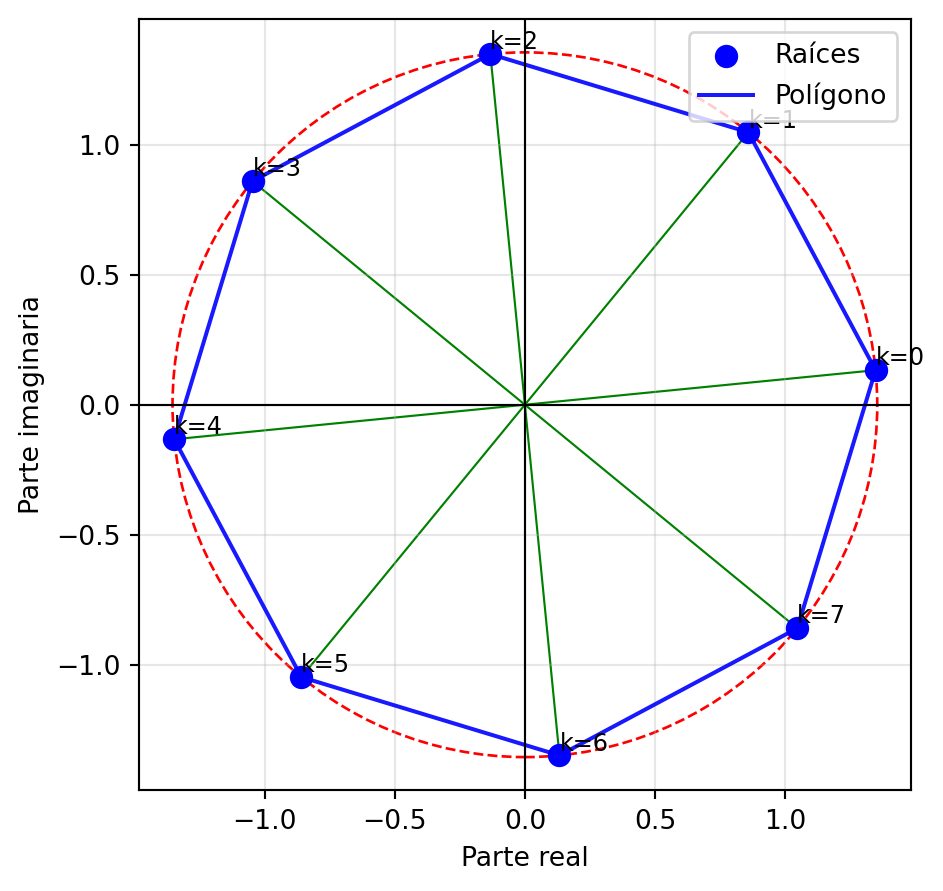
\includegraphics[keepaspectratio]{complejos-potenciacion-radicacion_files/figure-pdf/cell-4-output-1.pdf}}

\bookmarksetup{startatroot}

\chapter{Álgebra lineal}\label{uxe1lgebra-lineal}

\section{Ejemplo planteado:}\label{ejemplo-planteado}

Sea el sistema

\[
\begin{cases}
-2x-3y \;=\; 3,\\[2pt]
y \;=\; 1.
\end{cases}
\]

Hallar la inversa de coeficientes y resolver el sistema.

Dada su forma matricial, \(AX=B\):

\[
A=\begin{bmatrix}-2 & -3\\[2pt] 1 & 0\end{bmatrix},\quad
X=\begin{bmatrix}x\\[2pt] y\end{bmatrix},\quad
B=\begin{bmatrix}3\\[2pt] 1\end{bmatrix}.
\]

Planteamos la \textbf{inversa generica} y usamos \(A A^{-1} = 1\).
Obtenemos: \[
\begin{bmatrix}-2{\alpha}-3{\gamma} & -2{\beta}-3{\delta}\\[2pt] 0{\alpha}+1{\gamma} & 0{\beta}+1{\delta}\end{bmatrix}\quad=\begin{bmatrix}1 & 0\\[2pt] 0 & 1\end{bmatrix}\quad
\]

Entonces, se obtiene el sistema para
\({\alpha}, {\beta}, {\gamma},{\delta}\) \[
-2{\alpha}-3{\gamma} \;=\; 1,\\
-2{\beta}-3{\delta} \;=\; 0,\\
{\gamma} \;=\; 0.\\
{\delta} \;=\; 1.\
\] Sustituimos \({\gamma}\) y \({\delta}\): \[
-2{\alpha}-(3) · 0\;=\; 1,\\
-2{\beta}-(3) · 1\;=\; 0,\
\]

∴

\[
A^{-1}=\begin{bmatrix}-\tfrac{1}{2} & -\tfrac{3}{2}\\[2pt] 0 & 1\end{bmatrix}.
\]

Comprobacion rapida

\[
A A^{-1}=\begin{bmatrix}-2 & -3\\[2pt] 0 & 1\end{bmatrix} \
\begin{bmatrix}-\tfrac{1}{2} & -\tfrac{3}{2}\\[2pt] 0 & 1\end{bmatrix} =
\begin{bmatrix}1 & 0\\[2pt] 0 & 1\end{bmatrix}.
\]

Resolviendo \(X=A^{-1}B\): \[
\begin{bmatrix}x\\[2pt] y\end{bmatrix}=
\begin{bmatrix}-\tfrac{1}{2} & -\tfrac{3}{2}\\[2pt] 0 & 1\end{bmatrix}\begin{bmatrix}3\\[2pt] 1\end{bmatrix}
= \begin{bmatrix}-\tfrac{1}{2}· 3+-\tfrac{3}{2}· 1\\[2pt] 0· 3+1· 1\end{bmatrix}=\begin{bmatrix}-3\\[2pt] 1\end{bmatrix}
\] Por lo tanto,

\[
\boxed{\,x=-3,\qquad y=1}.
\]

\section{Diagonalización}\label{diagonalizaciuxf3n}

Ejercicio: \[
A=\begin{bmatrix}0 & -2\\[2pt] 1 & -3\end{bmatrix},\quad
\]

El polinomio característico de \(A\) es

\[
p_A(\lambda) = \det(A - \lambda I) = 
\det\!\begin{bmatrix}
-\lambda & 1\\
-2 & -3 - \lambda
\end{bmatrix}.\\
\\p_A(\lambda) = (-\lambda)(- 3 -\lambda) - (-2)(1)
= \lambda(\lambda + 3) + 2
= \lambda^2 + 3\lambda + 2.
\]

Factorizamos:

\[
p_A(\lambda) = (\lambda + 1)(\lambda + 2).
\]

\textbf{Valores propios: }

\[
\lambda_1 = -1, \qquad \lambda_2 = -2.
\]

\textbf{Espacio propio} de \(\lambda_1 = -1\)

Formamos \(A - (-1)I = A + I\):

\[
A + I = 
\begin{bmatrix}
1 & 1\\
-2 & -2
\end{bmatrix}.
\]

Resolvemos \((A + I)\)\(\vec{t} = 0\):

\[
\begin{bmatrix}1 & 1\\-2 & -2\end{bmatrix}
\begin{bmatrix}\vec{t}_1\\\vec{t}_2\end{bmatrix}
=\begin{bmatrix}0\\0\end{bmatrix}.
\]

Quiere decir que \(\vec{t}_1 = \vec{t}_2\),

Un \textbf{vector propio} asociado es:

\[
\mathbf{v}_1 =
\begin{bmatrix}
1\\
-1
\end{bmatrix}.
\]

Espacio propio de \(\lambda_2 = -2\)

Formamos \(A - (-2)I = A + 2I\):

\[
A + 2I = 
\begin{bmatrix}
2 & 1\\
-2 & -1
\end{bmatrix}.
\]

Resolvemos \((A + 2I)\vec{t} = 0\):

\[
\begin{bmatrix}
2 & 1\\
-2 & -1
\end{bmatrix}
\begin{bmatrix}
\vec{t}_1\\
\vec{t}_2
\end{bmatrix}
=
\begin{bmatrix}
0\\
0
\end{bmatrix}.
\]

Esto equivale a \(2\vec{t}_1 + \vec{t}_2 = 0\), es decir,
\(\vec{t}_2 = -2\vec{t}_1\).

Un \textbf{vector propio} asociado es:

\[
\mathbf{v}_2 =
\begin{bmatrix}
1\\
-2
\end{bmatrix}.
\]

\textbf{Construcción de} \(P\) y \(D\)

Colocamos los vectores propios como columnas de \(P\):

\[
P =
\begin{bmatrix}
1 & 1\\
-1 & -2
\end{bmatrix},
\qquad
D =
\begin{bmatrix}
-1 & 0\\
0 & -2
\end{bmatrix}.
\]

Comprobamos que se cumple:

\[
P^{-1}AP = D.
\] ∴ La matriz \(A\) es diagonalizable y hemos encontrado:

\[
A = P D P^{-1}, D = 
\text{diag}(-1, -2).
\]

\section{\texorpdfstring{Ejercicio matriz
\(3x3\)}{Ejercicio matriz 3x3}}\label{ejercicio-matriz-3x3}

\[
A=\begin{bmatrix}2 & 1 & 0\\[2pt] 0 & 2 & 0\\[2pt]\ 0 & 0 & 2\\[2pt]\end{bmatrix},\quad
\]

\section{Polinomio característico}\label{polinomio-caracteruxedstico}

El polinomio característico de \(A\) es \[
p_A(\lambda) = \det(A - \lambda I)
= \det
\begin{bmatrix}
2 - \lambda & 1 & 0\\
0 & 2 - \lambda & 0\\
0 & 0 & 2 - \lambda
\end{bmatrix}.
\]

Como la matriz es triangular superior, el determinante es el producto de
los elementos de la diagonal:

\[
p_A(\lambda) = (2 - \lambda)^3.
\]

Por lo tanto, el único valor propio es:

\[
\lambda = 2,
\]

con \textbf{multiplicidad algebraica} \[m_a = 3\].

\section{Vectores propios}\label{vectores-propios}

\textbf{Vectores propios}: Vamos a resolver

\[
(A - 2I)\vec{t} = 0,
\]

es decir,

\[
A - 2I =
\begin{bmatrix}
0 & 1 & 0\\
0 & 0 & 0\\
0 & 0 & 0
\end{bmatrix}.
\]

Sea
\(\vec{t} = \begin{bmatrix} \vec{t}_1 \\ \vec{t}_2 \\ \vec{t}_3 \end{bmatrix}\),
el sistema resulta:

\[
\vec{t}_2 = 0,
\]

con \(\vec{t}_1, \vec{t}_3\) libres. ∴

\[
\vec{t} =
\begin{bmatrix}
\vec{t}_1\\
0\\
\vec{t}_3
\end{bmatrix}
= \vec{t}_1
\begin{bmatrix}
1\\
0\\
0
\end{bmatrix}
+ \vec{t}_3
\begin{bmatrix}
0\\
0\\
1
\end{bmatrix}.
\]

\textbf{Espacio propio}: El espacio propio asociado a \(\lambda = 2\)
está generado por:

\[
\mathbf{v}_1 =
\begin{bmatrix}
1\\
0\\
0
\end{bmatrix},
\qquad
\mathbf{v}_2 =
\begin{bmatrix}
0\\
0\\
1
\end{bmatrix}.
\]

∴, \(A\) \textbf{no es diagonalizable} (solo tiene dos vectores propios
linealmente independientes para una matriz de orden 3).

\begin{center}\rule{0.5\linewidth}{0.5pt}\end{center}

\section{Comprobación computacional en
Python}\label{comprobaciuxf3n-computacional-en-python}

\begin{Shaded}
\begin{Highlighting}[]
\CommentTok{\# EDITA AQUÍ (1): MATRIZ A}
\NormalTok{A\_list }\OperatorTok{=}\NormalTok{ [}
\NormalTok{    [}\DecValTok{2}\NormalTok{, }\DecValTok{1}\NormalTok{, }\DecValTok{0}\NormalTok{],}
\NormalTok{    [}\DecValTok{0}\NormalTok{, }\DecValTok{2}\NormalTok{, }\DecValTok{0}\NormalTok{],}
\NormalTok{    [}\DecValTok{0}\NormalTok{, }\DecValTok{0}\NormalTok{, }\DecValTok{2}\NormalTok{],}
\NormalTok{]}

\CommentTok{\# EDITA AQUÍ (2): eigenvalor a analizar}
\NormalTok{lambda\_eval }\OperatorTok{=} \DecValTok{2}

\ImportTok{import}\NormalTok{ sympy }\ImportTok{as}\NormalTok{ sp}

\NormalTok{A }\OperatorTok{=}\NormalTok{ sp.Matrix(A\_list)}
\NormalTok{n }\OperatorTok{=}\NormalTok{ A.shape[}\DecValTok{0}\NormalTok{]}

\BuiltInTok{print}\NormalTok{(}\StringTok{"Matriz A ="}\NormalTok{)}
\NormalTok{sp.pprint(A)}\OperatorTok{;} \BuiltInTok{print}\NormalTok{()}

\CommentTok{\# 1) Valores propios y multiplicidades algebraicas}
\NormalTok{evals }\OperatorTok{=}\NormalTok{ A.eigenvals()}
\BuiltInTok{print}\NormalTok{(}\StringTok{"Valores propios (m\_a):"}\NormalTok{)}
\ControlFlowTok{for}\NormalTok{ lam, mult }\KeywordTok{in}\NormalTok{ evals.items():}
    \BuiltInTok{print}\NormalTok{(}\SpecialStringTok{f"  λ = }\SpecialCharTok{\{}\NormalTok{lam}\SpecialCharTok{\}}\SpecialStringTok{   (m\_a = }\SpecialCharTok{\{}\NormalTok{mult}\SpecialCharTok{\}}\SpecialStringTok{)"}\NormalTok{)}
\BuiltInTok{print}\NormalTok{()}

\CommentTok{\# 2) Espacio propio de lambda\_eval}
\NormalTok{E }\OperatorTok{=}\NormalTok{ A }\OperatorTok{{-}}\NormalTok{ lambda\_eval}\OperatorTok{*}\NormalTok{sp.eye(n)}
\BuiltInTok{print}\NormalTok{(}\SpecialStringTok{f"Espacio propio para λ = }\SpecialCharTok{\{}\NormalTok{lambda\_eval}\SpecialCharTok{\}}\SpecialStringTok{:  (A {-} λI) v = 0"}\NormalTok{)}
\BuiltInTok{print}\NormalTok{(}\StringTok{"A {-} λI ="}\NormalTok{)}
\NormalTok{sp.pprint(E)}\OperatorTok{;} \BuiltInTok{print}\NormalTok{()}

\NormalTok{null\_basis }\OperatorTok{=}\NormalTok{ E.nullspace()}
\BuiltInTok{print}\NormalTok{(}\StringTok{"Base del espacio propio:"}\NormalTok{)}
\ControlFlowTok{if}\NormalTok{ null\_basis:}
    \ControlFlowTok{for}\NormalTok{ i, v }\KeywordTok{in} \BuiltInTok{enumerate}\NormalTok{(null\_basis, }\DecValTok{1}\NormalTok{):}
        \BuiltInTok{print}\NormalTok{(}\SpecialStringTok{f"  v\_}\SpecialCharTok{\{}\NormalTok{i}\SpecialCharTok{\}}\SpecialStringTok{ = "}\NormalTok{)}\OperatorTok{;}\NormalTok{ sp.pprint(v)}\OperatorTok{;} \BuiltInTok{print}\NormalTok{()}
\ControlFlowTok{else}\NormalTok{:}
    \BuiltInTok{print}\NormalTok{(}\StringTok{"  (vacío) → λ no es eigenvalor de A}\CharTok{\textbackslash{}n}\StringTok{"}\NormalTok{)}

\NormalTok{m\_g }\OperatorTok{=} \BuiltInTok{len}\NormalTok{(null\_basis)}
\BuiltInTok{print}\NormalTok{(}\SpecialStringTok{f"Multiplicidad geométrica m\_g(λ=}\SpecialCharTok{\{}\NormalTok{lambda\_eval}\SpecialCharTok{\}}\SpecialStringTok{) = }\SpecialCharTok{\{}\NormalTok{m\_g}\SpecialCharTok{\}}\CharTok{\textbackslash{}n}\SpecialStringTok{"}\NormalTok{)}

\CommentTok{\# 3) ¿Es A diagonalizable? (suma de m\_g para todos los λ debe ser n)}
\NormalTok{eig\_vects }\OperatorTok{=}\NormalTok{ A.eigenvects()  }\CommentTok{\# [(λ, m\_a, [basis]), ...]}
\NormalTok{total\_geom }\OperatorTok{=} \BuiltInTok{sum}\NormalTok{(}\BuiltInTok{len}\NormalTok{(basis) }\ControlFlowTok{for}\NormalTok{ \_, \_, basis }\KeywordTok{in}\NormalTok{ eig\_vects)}
\NormalTok{es\_diag }\OperatorTok{=}\NormalTok{ (total\_geom }\OperatorTok{==}\NormalTok{ n)}

\BuiltInTok{print}\NormalTok{(}\StringTok{"¿A es diagonalizable?"}\NormalTok{)}
\BuiltInTok{print}\NormalTok{(}\SpecialStringTok{f"  Suma de multiplicidades geométricas = }\SpecialCharTok{\{}\NormalTok{total\_geom}\SpecialCharTok{\}}\SpecialStringTok{ (n = }\SpecialCharTok{\{}\NormalTok{n}\SpecialCharTok{\}}\SpecialStringTok{)"}\NormalTok{)}
\BuiltInTok{print}\NormalTok{(}\SpecialStringTok{f"  Resultado: }\SpecialCharTok{\{}\StringTok{\textquotesingle{}SÍ\textquotesingle{}} \ControlFlowTok{if}\NormalTok{ es\_diag }\ControlFlowTok{else} \StringTok{\textquotesingle{}NO\textquotesingle{}}\SpecialCharTok{\}}\CharTok{\textbackslash{}n}\SpecialStringTok{"}\NormalTok{)}

\CommentTok{\# 4) Si es diagonalizable, construimos P y D y verificamos P\^{}\{{-}1\} A P = D}
\ControlFlowTok{if}\NormalTok{ es\_diag:}
\NormalTok{    eig\_vects\_sorted }\OperatorTok{=} \BuiltInTok{sorted}\NormalTok{(eig\_vects, key}\OperatorTok{=}\KeywordTok{lambda}\NormalTok{ t: t[}\DecValTok{0}\NormalTok{])  }\CommentTok{\# ordenar por λ (opcional)}
\NormalTok{    P\_cols, D\_diag }\OperatorTok{=}\NormalTok{ [], []}
    \ControlFlowTok{for}\NormalTok{ lam, \_, basis }\KeywordTok{in}\NormalTok{ eig\_vects\_sorted:}
        \ControlFlowTok{for}\NormalTok{ v }\KeywordTok{in}\NormalTok{ basis:}
\NormalTok{            P\_cols.append(sp.Matrix(v))}
\NormalTok{            D\_diag.append(lam)}
\NormalTok{    P }\OperatorTok{=}\NormalTok{ sp.Matrix.hstack(}\OperatorTok{*}\NormalTok{P\_cols)}
\NormalTok{    D }\OperatorTok{=}\NormalTok{ sp.diag(}\OperatorTok{*}\NormalTok{D\_diag)}

    \BuiltInTok{print}\NormalTok{(}\StringTok{"P (columnas = eigenvectores):"}\NormalTok{)}
\NormalTok{    sp.pprint(P)}\OperatorTok{;} \BuiltInTok{print}\NormalTok{()}
    \BuiltInTok{print}\NormalTok{(}\StringTok{"D (diagonal de eigenvalores):"}\NormalTok{)}
\NormalTok{    sp.pprint(D)}\OperatorTok{;} \BuiltInTok{print}\NormalTok{()}

    \BuiltInTok{print}\NormalTok{(}\StringTok{"Verificación P\^{}\{{-}1\} A P ="}\NormalTok{)}
\NormalTok{    sp.pprint(sp.simplify(P.inv()}\OperatorTok{*}\NormalTok{A}\OperatorTok{*}\NormalTok{P))}\OperatorTok{;} \BuiltInTok{print}\NormalTok{()}
\ControlFlowTok{else}\NormalTok{:}
    \BuiltInTok{print}\NormalTok{(}\StringTok{"Explicación:"}\NormalTok{)}
    \BuiltInTok{print}\NormalTok{(}\StringTok{"  No hay suficientes eigenvectores linealmente independientes para formar P."}\NormalTok{)}
\end{Highlighting}
\end{Shaded}

\begin{verbatim}
Matriz A =
⎡2  1  0⎤
⎢       ⎥
⎢0  2  0⎥
⎢       ⎥
⎣0  0  2⎦

Valores propios (m_a):
  λ = 2   (m_a = 3)

Espacio propio para λ = 2:  (A - λI) v = 0
A - λI =
⎡0  1  0⎤
⎢       ⎥
⎢0  0  0⎥
⎢       ⎥
⎣0  0  0⎦

Base del espacio propio:
  v_1 = 
⎡1⎤
⎢ ⎥
⎢0⎥
⎢ ⎥
⎣0⎦

  v_2 = 
⎡0⎤
⎢ ⎥
⎢0⎥
⎢ ⎥
⎣1⎦

Multiplicidad geométrica m_g(λ=2) = 2

¿A es diagonalizable?
  Suma de multiplicidades geométricas = 2 (n = 3)
  Resultado: NO

Explicación:
  No hay suficientes eigenvectores linealmente independientes para formar P.
\end{verbatim}

\bookmarksetup{startatroot}

\chapter{Ecuaciones en diferencia y métodos de
aproximación}\label{ecuaciones-en-diferencia-y-muxe9todos-de-aproximaciuxf3n}

\section{Método de Herón para aproximar raíces
cuadradas}\label{muxe9todo-de-heruxf3n-para-aproximar-rauxedces-cuadradas}

El \textbf{método de Herón}, también llamado método babilónico, es un
procedimiento iterativo para calcular raíces cuadradas.\\
Dado un número ( S ) y una estimación inicial ( y\_0 ), la fórmula
general es:

\[
y(k+1) = \frac{1}{2}\left(y_k + \frac{S}{y_k}\right)
\]

Cada iteración mejora la aproximación al valor real \sqrt(S).\\
El proceso se basa en una idea equivalente al método de Newton aplicado
a \[
f(y) = y^2 - S 
\] La iteración se detiene cuando la diferencia ( \textbar y\_\{k+1\} -
y\_k\textbar{} ) es suficientemente pequeña.

\section{\texorpdfstring{Ejemplo aproximación de raiz cuadrada de 2 con
\(y0=1\)}{Ejemplo aproximación de raiz cuadrada de 2 con y0=1}}\label{ejemplo-aproximaciuxf3n-de-raiz-cuadrada-de-2-con-y01}

Aplicando el método:

{[}

\begin{aligned}
y_1 &= \tfrac{1}{2}(1 + 2/1) = 1.5,\\[4pt]
y_2 &= \tfrac{1}{2}(1.5 + 2/1.5) = 1.4166,\\[4pt]
y_3 &= \tfrac{1}{2}(1.4166 + 2/1.4166) = 1.4142.
\end{aligned}

{]}

Con solo tres iteraciones, el resultado se aproxima al valor real:

raiz de 2 = 1.41421356

Al elevar ( 1.4142\^{}2 ) se obtiene aproximadamente ( 2 ), confirmando
la exactitud de la aproximación.

\section{Ecuación en diferencia tipo
Fibonacci}\label{ecuaciuxf3n-en-diferencia-tipo-fibonacci}

Consideremos la ecuación en diferencia:

\[
y_{n+2} - y_{n+1} - y_n = 0, 
\qquad y_0 = 1,\; y_1 = 1.
\]

Su polinomio característico es: \[
r^2 - r - 1 = 0.
\]

Sus raíces son: \[
r_1 = \frac{1 + \sqrt{5}}{2}, 
\qquad 
r_2 = \frac{1 - \sqrt{5}}{2}.
\] Por lo tanto, la solución general es: \[
y_n = A\,r_1^n + B\,r_2^n.
\]

Aplicando las condiciones iniciales, se obtiene la \textbf{forma cerrada
de Fibonacci}: \[
y_n = \frac{r_1^{\,n+1} - r_2^{\,n+1}}{\sqrt{5}}.
\]

\section{Método general para ecuaciones en diferencia lineales con
coeficientes
constantes}\label{muxe9todo-general-para-ecuaciones-en-diferencia-lineales-con-coeficientes-constantes}

Para una ecuación de orden (k): \[
a_k y_{n+k} + a_{k-1} y_{n+k-1} + \dots + a_0 y_n = g(n),
\]

los pasos generales son:

\begin{enumerate}
\def\labelenumi{\arabic{enumi}.}
\tightlist
\item
  Plantear la \textbf{ecuación característica} (caso homogéneo ( g(n) =
  0 )).\\
\item
  Encontrar las \textbf{raíces} del polinomio y su multiplicidad.\\
\item
  Formar la \textbf{solución homogénea} según el tipo de raíces (reales,
  repetidas o complejas).\\
\item
  Proponer una \textbf{solución particular} dependiendo de ( g(n) ).\\
\item
  Sumar ambas y aplicar \textbf{condiciones iniciales} para determinar
  las constantes.
\end{enumerate}

\section{Ejemplo no homogéneo}\label{ejemplo-no-homoguxe9neo}

\[
y_{n+2} - 3y_{n+1} + 2y_n = 4^n, 
\qquad 
y_0 = 0,\; y_1 = 4.
\]

Ecuación característica: \[
r^2 - 3r + 2 = 0 
\quad \Rightarrow \quad 
r = 1,\; 2.
\]

Solución homogénea: \[
y_n^{(h)} = A + B\,2^n.
\]

Propuesta particular: \[
y_n^{(p)} = C\,4^n \quad \Rightarrow \quad C = \frac{1}{6}.
\]

Solución general: \[
y_n = A + B\,2^n + \tfrac{1}{6}4^n.
\]

Determinando las constantes con \(y_0\) y \(y_1\), se obtiene la
secuencia final.

\section{Interpretación
computacional}\label{interpretaciuxf3n-computacional}

Las ecuaciones en diferencia pueden implementarse fácilmente en código
para simular sus valores iterativos.

\textbf{Ejemplo 1 --- Método de Herón:}

\begin{Shaded}
\begin{Highlighting}[]
\KeywordTok{def}\NormalTok{ heron\_sqrt(S, y0}\OperatorTok{=}\FloatTok{1.0}\NormalTok{, tol}\OperatorTok{=}\FloatTok{1e{-}10}\NormalTok{, max\_iter}\OperatorTok{=}\DecValTok{10}\NormalTok{):}
    \CommentTok{"""}
\CommentTok{    Aproxima la raíz cuadrada de S mediante el método de Herón.}
\CommentTok{    """}
\NormalTok{    y }\OperatorTok{=}\NormalTok{ y0}
    \ControlFlowTok{for}\NormalTok{ \_ }\KeywordTok{in} \BuiltInTok{range}\NormalTok{(max\_iter):}
\NormalTok{        y\_next }\OperatorTok{=} \FloatTok{0.5} \OperatorTok{*}\NormalTok{ (y }\OperatorTok{+}\NormalTok{ S }\OperatorTok{/}\NormalTok{ y)}
        \ControlFlowTok{if} \BuiltInTok{abs}\NormalTok{(y\_next }\OperatorTok{{-}}\NormalTok{ y) }\OperatorTok{\textless{}}\NormalTok{ tol:}
            \ControlFlowTok{break}
\NormalTok{        y }\OperatorTok{=}\NormalTok{ y\_next}
    \ControlFlowTok{return}\NormalTok{ y}
\BuiltInTok{print}\NormalTok{(}\StringTok{"Aproximación de sqrt(2):"}\NormalTok{, heron\_sqrt(}\DecValTok{2}\NormalTok{))}
\end{Highlighting}
\end{Shaded}

\begin{verbatim}
Aproximación de sqrt(2): 1.4142135623746899
\end{verbatim}

\textbf{Ejemplo 2 --- Ecuación en diferencia no homogénea:}

\begin{Shaded}
\begin{Highlighting}[]
\KeywordTok{def}\NormalTok{ solve\_second\_order(a1, a0, g, y0, y1, N):}
    \CommentTok{"""}
\CommentTok{    Resuelve una ecuación en diferencia del tipo:}
\CommentTok{        y\_\{n+2\} + a1*y\_\{n+1\} + a0*y\_n = g(n)}
\CommentTok{    """}
\NormalTok{    y }\OperatorTok{=}\NormalTok{ [y0, y1]}
    \ControlFlowTok{for}\NormalTok{ n }\KeywordTok{in} \BuiltInTok{range}\NormalTok{(}\DecValTok{0}\NormalTok{, N}\OperatorTok{{-}}\DecValTok{2}\NormalTok{):}
\NormalTok{        y\_next }\OperatorTok{=} \OperatorTok{{-}}\NormalTok{a1 }\OperatorTok{*}\NormalTok{ y[}\OperatorTok{{-}}\DecValTok{1}\NormalTok{] }\OperatorTok{{-}}\NormalTok{ a0 }\OperatorTok{*}\NormalTok{ y[}\OperatorTok{{-}}\DecValTok{2}\NormalTok{] }\OperatorTok{+}\NormalTok{ g(n)}
\NormalTok{        y.append(y\_next)}
    \ControlFlowTok{return}\NormalTok{ y}

\CommentTok{\# Ejemplo con y\_\{n+2\} {-} 3y\_\{n+1\} + 2y\_n = 4\^{}n}
\NormalTok{g }\OperatorTok{=} \KeywordTok{lambda}\NormalTok{ n: }\DecValTok{4}\OperatorTok{**}\NormalTok{n}
\NormalTok{seq }\OperatorTok{=}\NormalTok{ solve\_second\_order(}\OperatorTok{{-}}\DecValTok{3}\NormalTok{, }\DecValTok{2}\NormalTok{, g, y0}\OperatorTok{=}\DecValTok{0}\NormalTok{, y1}\OperatorTok{=}\DecValTok{4}\NormalTok{, N}\OperatorTok{=}\DecValTok{8}\NormalTok{)}
\BuiltInTok{print}\NormalTok{(}\StringTok{"Secuencia y\_n:"}\NormalTok{, seq)}
\end{Highlighting}
\end{Shaded}

\begin{verbatim}
Secuencia y_n: [0, 4, 13, 35, 95, 279, 903, 3175]
\end{verbatim}

\section{Conclusión}\label{conclusiuxf3n}

Las ecuaciones en diferencia constituyen una herramienta fundamental
para modelar \textbf{procesos discretos} y \textbf{series temporales},
con aplicaciones en economía, ingeniería y algoritmos de aprendizaje.\\
El método de Herón, por su parte, ejemplifica el poder de los
procedimientos iterativos para alcanzar soluciones precisas a partir de
aproximaciones iniciales simples.

\bookmarksetup{startatroot}

\chapter{Ecuaciones en diferencia y
finanzas}\label{ecuaciones-en-diferencia-y-finanzas}

\section{Valor futuro y fórmulas
financieras}\label{valor-futuro-y-fuxf3rmulas-financieras}

El valor futuro (F) de una inversión (P) a una tasa de interés (i)
durante (n) períodos se expresa como:

\[
F=P(1+i)^n
\] Cada período multiplica el capital por \((1+i)\).\\
La relación entre períodos consecutivos puede verse como: \[
F_n = (1+i)F_{n-1},
\]

una ecuación en diferencia que representa crecimiento exponencial
discreto.

\section{Del interés compuesto a la ecuación en
diferencia}\label{del-interuxe9s-compuesto-a-la-ecuaciuxf3n-en-diferencia}

El modelo discreto: \[
F_{n+1} = (1+i)F_n
\]

describe el interés compuesto acumulativo.\\
Si \((i = 0.1)\) y \((F_0 = 1000)\):\\
\[
(F_1 = 1100,; F_2 = 1210,\; F_3 = 1331, \dots\
\] Esta forma recursiva permite analizar o simular el comportamiento del
dinero a lo largo del tiempo.

\section{Ventajas del enfoque con ecuaciones en
diferencia}\label{ventajas-del-enfoque-con-ecuaciones-en-diferencia}

\begin{itemize}
\tightlist
\item
  Permite observar la \textbf{evolución temporal} del capital paso a
  paso.\\
\item
  Facilita la \textbf{simulación} mediante algoritmos iterativos.\\
\item
  Acepta \textbf{términos variables}, como aportes o retiros
  periódicos.\\
\item
  Se adapta a análisis predictivos y de \textbf{riesgo financiero}.
\end{itemize}

\section{Modelos financieros como ecuaciones en
diferencia}\label{modelos-financieros-como-ecuaciones-en-diferencia}

\textbf{Interés compuesto:} \[
F_{n+1} = (1+i)F_n
\]

\textbf{Serie uniforme (aportes constantes (A)):} \[
F_{n+1} = (1+i)F_n + A
\]

\textbf{Serie con gradiente aritmético:} \[
F_{n+1} = (1+i)F_n + (A + Gn),
\]

donde \(G\) es el cambio progresivo en los pagos.\\
Cada uno representa una variación del modelo general de crecimiento
financiero discreto.

\section{Simulación de modelos
financieros}\label{simulaciuxf3n-de-modelos-financieros}

Ejemplo de \textbf{interés compuesto}:

\begin{Shaded}
\begin{Highlighting}[]
\NormalTok{F }\OperatorTok{=} \DecValTok{1000}
\NormalTok{i }\OperatorTok{=} \FloatTok{0.1}
\ControlFlowTok{for}\NormalTok{ n }\KeywordTok{in} \BuiltInTok{range}\NormalTok{(}\DecValTok{5}\NormalTok{):}
\NormalTok{    F }\OperatorTok{=}\NormalTok{ (}\DecValTok{1} \OperatorTok{+}\NormalTok{ i) }\OperatorTok{*}\NormalTok{ F}
    \BuiltInTok{print}\NormalTok{(}\SpecialStringTok{f"Periodo }\SpecialCharTok{\{}\NormalTok{n}\OperatorTok{+}\DecValTok{1}\SpecialCharTok{\}}\SpecialStringTok{: F = }\SpecialCharTok{\{}\NormalTok{F}\SpecialCharTok{:.2f\}}\SpecialStringTok{"}\NormalTok{)}
\end{Highlighting}
\end{Shaded}

\begin{verbatim}
Periodo 1: F = 1100.00
Periodo 2: F = 1210.00
Periodo 3: F = 1331.00
Periodo 4: F = 1464.10
Periodo 5: F = 1610.51
\end{verbatim}

Ejemplo de \textbf{serie uniforme}:

\begin{Shaded}
\begin{Highlighting}[]
\NormalTok{F }\OperatorTok{=} \DecValTok{0}
\NormalTok{i }\OperatorTok{=} \FloatTok{0.08}
\NormalTok{A }\OperatorTok{=} \DecValTok{200}
\ControlFlowTok{for}\NormalTok{ n }\KeywordTok{in} \BuiltInTok{range}\NormalTok{(}\DecValTok{6}\NormalTok{):}
\NormalTok{    F }\OperatorTok{=}\NormalTok{ (}\DecValTok{1} \OperatorTok{+}\NormalTok{ i) }\OperatorTok{*}\NormalTok{ F }\OperatorTok{+}\NormalTok{ A}
    \BuiltInTok{print}\NormalTok{(}\SpecialStringTok{f"Periodo }\SpecialCharTok{\{}\NormalTok{n}\OperatorTok{+}\DecValTok{1}\SpecialCharTok{\}}\SpecialStringTok{: F = }\SpecialCharTok{\{}\NormalTok{F}\SpecialCharTok{:.2f\}}\SpecialStringTok{"}\NormalTok{)}
\end{Highlighting}
\end{Shaded}

\begin{verbatim}
Periodo 1: F = 200.00
Periodo 2: F = 416.00
Periodo 3: F = 649.28
Periodo 4: F = 901.22
Periodo 5: F = 1173.32
Periodo 6: F = 1467.19
\end{verbatim}

Estas simulaciones reproducen exactamente la ecuación en diferencia
asociada a cada modelo.

\section{Interpretación dinámica del valor del
dinero}\label{interpretaciuxf3n-dinuxe1mica-del-valor-del-dinero}

La ecuación: \[
F_{n+1} - F_n = iF_n
\] muestra que el cambio de un período a otro es proporcional al capital
actual.\\
Representa un \textbf{crecimiento exponencial discreto}, donde el dinero
genera más valor conforme aumenta.\\
Este enfoque permite modelar fenómenos financieros como inversiones,
préstamos o inflación en el tiempo.

\bookmarksetup{startatroot}

\chapter{Ecuaciones logísticas y dinámica
poblacional}\label{ecuaciones-loguxedsticas-y-dinuxe1mica-poblacional}

\section{Introducción al modelo logístico
discreto}\label{introducciuxf3n-al-modelo-loguxedstico-discreto}

El \textbf{modelo logístico discreto} describe la evolución de una
población que crece con una tasa limitada por la competencia interna.\\
La ecuación básica es: \[
x_{n+1} = r\,x_n(1 - x_n)
\]

donde: - \(x_n\): población normalizada (entre 0 y 1), - \(r\):
parámetro de crecimiento o tasa de reproducción, - \(x_{n+1}\):
población en el siguiente período.

Este modelo capta cómo una población aumenta rápidamente al principio,
pero se estabiliza cuando se acerca al límite de recursos.\\
Fue propuesto originalmente por \textbf{Pierre-François Verhulst (1845)}
y es un ejemplo clásico de \textbf{modelo no lineal discreto}.

\section{Modelo logístico de la población de
conejos}\label{modelo-loguxedstico-de-la-poblaciuxf3n-de-conejos}

Supongamos una población de \textbf{conejos} en un ambiente con recursos
limitados.\\
Si \(x_n\) representa la proporción de conejos respecto a la capacidad
máxima del entorno y \(r\) es la tasa de crecimiento, la evolución está
dada por:

\[
x_{n+1} = r\,x_n(1 - x_n)
\]

Este modelo genera distintos comportamientos dependiendo del valor de
\(r\): - Si \(r < 1\): la población desaparece (tiende a 0). - Si
\(1 < r < 3\): la población se estabiliza en un valor fijo. - Si
\(3 < r < 3.57\): aparecen \textbf{ciclos} de período 2, 4, 8, etc. - Si
\(r > 3.57\): la población entra en \textbf{caos}.

\section{Implementación en Python del modelo de
conejos}\label{implementaciuxf3n-en-python-del-modelo-de-conejos}

\begin{Shaded}
\begin{Highlighting}[]
\ImportTok{import}\NormalTok{ numpy }\ImportTok{as}\NormalTok{ np}
\ImportTok{import}\NormalTok{ matplotlib.pyplot }\ImportTok{as}\NormalTok{ plt}

\KeywordTok{def}\NormalTok{ logistic\_population(r, x0, n):}
\NormalTok{    x }\OperatorTok{=}\NormalTok{ np.zeros(n)}
\NormalTok{    x[}\DecValTok{0}\NormalTok{] }\OperatorTok{=}\NormalTok{ x0}
    \ControlFlowTok{for}\NormalTok{ i }\KeywordTok{in} \BuiltInTok{range}\NormalTok{(}\DecValTok{1}\NormalTok{, n):}
\NormalTok{        x[i] }\OperatorTok{=}\NormalTok{ r }\OperatorTok{*}\NormalTok{ x[i}\OperatorTok{{-}}\DecValTok{1}\NormalTok{] }\OperatorTok{*}\NormalTok{ (}\DecValTok{1} \OperatorTok{{-}}\NormalTok{ x[i}\OperatorTok{{-}}\DecValTok{1}\NormalTok{])}
    \ControlFlowTok{return}\NormalTok{ x}

\CommentTok{\# Parámetros}
\NormalTok{r }\OperatorTok{=} \FloatTok{3.9}
\NormalTok{x0 }\OperatorTok{=} \FloatTok{0.2}
\NormalTok{n }\OperatorTok{=} \DecValTok{100}
\NormalTok{x }\OperatorTok{=}\NormalTok{ logistic\_population(r, x0, n)}

\NormalTok{plt.plot(}\BuiltInTok{range}\NormalTok{(n), x, lw}\OperatorTok{=}\FloatTok{1.5}\NormalTok{)}
\NormalTok{plt.title(}\SpecialStringTok{f"Modelo logístico de población de conejos (r=}\SpecialCharTok{\{}\NormalTok{r}\SpecialCharTok{\}}\SpecialStringTok{)"}\NormalTok{)}
\NormalTok{plt.xlabel(}\StringTok{"Generación n"}\NormalTok{)}
\NormalTok{plt.ylabel(}\StringTok{"Población normalizada xₙ"}\NormalTok{)}
\NormalTok{plt.show()}
\end{Highlighting}
\end{Shaded}

\pandocbounded{\includegraphics[keepaspectratio]{ecuaciones-logisticas_files/figure-pdf/cell-2-output-1.pdf}}

\textbf{Interpretación:}\\
- Para (r=2.5), la población converge a un valor estable.\\
- Para (r=3.2), oscila entre dos niveles.\\
- Para (r=3.9), el comportamiento es caótico.

\begin{center}\rule{0.5\linewidth}{0.5pt}\end{center}

\section{Evolución temporal y sensibilidad a las condiciones
iniciales}\label{evoluciuxf3n-temporal-y-sensibilidad-a-las-condiciones-iniciales}

El modelo presenta \textbf{sensibilidad a las condiciones iniciales}:\\
si \((x_0 = 0.2000)\) y \((x_0' = 0.2001)\), la diferencia entre ambas
trayectorias puede crecer exponencialmente para valores altos de \(r\).

Esta propiedad es una característica del \textbf{caos determinista},
donde el sistema sigue una regla exacta pero el resultado se vuelve
impredecible.

\section{Diagrama de telaraña (Cobweb
plot)}\label{diagrama-de-telarauxf1a-cobweb-plot}

El \textbf{diagrama de telaraña} permite visualizar gráficamente la
evolución de la población:

\begin{enumerate}
\def\labelenumi{\arabic{enumi}.}
\tightlist
\item
  Se dibuja la curva \(y = r\,x(1 - x)\) y la recta \(y = x\).
\item
  Se parte desde un punto inicial \(x_0\).
\item
  Se sube a la curva (para obtener \(x_1\)) y luego se proyecta a la
  recta identidad (para regresar al eje x).
\item
  Repitiendo el proceso se genera una figura que muestra cómo evoluciona
  la población.
\end{enumerate}

\textbf{Interpretación:}\\
- Si el trazado converge al punto fijo, el sistema es estable.\\
- Si alterna entre varios valores, existe un ciclo periódico.\\
- Si no hay patrón repetido, el sistema es caótico.

\section{Diagrama de bifurcación}\label{diagrama-de-bifurcaciuxf3n}

El \textbf{diagrama de bifurcación} muestra el comportamiento de largo
plazo de la ecuación logística al variar el parámetro \(r\).

Para cada valor de \(r\), se calculan muchas iteraciones y se grafican
los valores finales de \(x_n\).

\begin{itemize}
\tightlist
\item
  \(r < 1\): la población muere.
\item
  \(1 < r < 3\): la población se estabiliza.
\item
  \(3 < r < 3.57\): se duplican los períodos (2, 4, 8\ldots).
\item
  \(r > 3.57\): el sistema entra en caos.
\end{itemize}

La secuencia de duplicaciones de período obedece a la \textbf{constante
de Feigenbaum (\(\delta \approx 4.6692\))}, que describe la relación
entre los intervalos sucesivos de bifurcación.

\begin{Shaded}
\begin{Highlighting}[]
\KeywordTok{def}\NormalTok{ bifurcation(r\_min}\OperatorTok{=}\FloatTok{2.5}\NormalTok{, r\_max}\OperatorTok{=}\FloatTok{4.0}\NormalTok{, steps}\OperatorTok{=}\DecValTok{3000}\NormalTok{, transient}\OperatorTok{=}\DecValTok{200}\NormalTok{, plot\_points}\OperatorTok{=}\DecValTok{200}\NormalTok{):}
\NormalTok{    rs }\OperatorTok{=}\NormalTok{ np.linspace(r\_min, r\_max, steps)}
\NormalTok{    xs }\OperatorTok{=}\NormalTok{ []}
\NormalTok{    rs\_all }\OperatorTok{=}\NormalTok{ []}
    \ControlFlowTok{for}\NormalTok{ r }\KeywordTok{in}\NormalTok{ rs:}
\NormalTok{        x }\OperatorTok{=} \FloatTok{0.5}
        \ControlFlowTok{for}\NormalTok{ \_ }\KeywordTok{in} \BuiltInTok{range}\NormalTok{(transient):}
\NormalTok{            x }\OperatorTok{=}\NormalTok{ r }\OperatorTok{*}\NormalTok{ x }\OperatorTok{*}\NormalTok{ (}\DecValTok{1} \OperatorTok{{-}}\NormalTok{ x)}
        \ControlFlowTok{for}\NormalTok{ \_ }\KeywordTok{in} \BuiltInTok{range}\NormalTok{(plot\_points):}
\NormalTok{            x }\OperatorTok{=}\NormalTok{ r }\OperatorTok{*}\NormalTok{ x }\OperatorTok{*}\NormalTok{ (}\DecValTok{1} \OperatorTok{{-}}\NormalTok{ x)}
\NormalTok{            xs.append(x)}
\NormalTok{            rs\_all.append(r)}
\NormalTok{    plt.figure(figsize}\OperatorTok{=}\NormalTok{(}\DecValTok{8}\NormalTok{,}\DecValTok{6}\NormalTok{))}
\NormalTok{    plt.scatter(rs\_all, xs, s}\OperatorTok{=}\FloatTok{0.1}\NormalTok{, color}\OperatorTok{=}\StringTok{"blue"}\NormalTok{)}
\NormalTok{    plt.title(}\StringTok{"Diagrama de bifurcación del mapa logístico"}\NormalTok{)}
\NormalTok{    plt.xlabel(}\StringTok{"Parámetro r"}\NormalTok{)}
\NormalTok{    plt.ylabel(}\StringTok{"xₙ"}\NormalTok{)}
\NormalTok{    plt.show()}

\NormalTok{bifurcation()}
\end{Highlighting}
\end{Shaded}

\pandocbounded{\includegraphics[keepaspectratio]{ecuaciones-logisticas_files/figure-pdf/cell-3-output-1.pdf}}

\section{\texorpdfstring{Ejemplos de comportamiento según el valor de
\(r\)}{Ejemplos de comportamiento según el valor de r}}\label{ejemplos-de-comportamiento-seguxfan-el-valor-de-r}

\begin{longtable}[]{@{}lll@{}}
\toprule\noalign{}
Valor de \(r\) & Tipo de comportamiento & Descripción breve \\
\midrule\noalign{}
\endhead
\bottomrule\noalign{}
\endlastfoot
2.5 & Estable & Convergencia a punto fijo \(x^* = 1 - 1/r = 0.6\). \\
3.2 & Período 2 & Alternancia entre dos valores. \\
3.5 & Período 4 o 8 & Ciclo de mayor complejidad. \\
3.9 & Caótico & Trayectorias impredecibles y sensibles a \(x_0\). \\
\end{longtable}

\section{Relación con el algoritmo de Shor y
periodicidad}\label{relaciuxf3n-con-el-algoritmo-de-shor-y-periodicidad}

El \textbf{algoritmo de Shor} (usado en computación cuántica para
factorización) busca el \textbf{período} de una función modular:

\[
f(a) = r^a \bmod N
\]

donde \(N\) es el número a factorizar y \(r\) es una base coprima con
\(N\).\\
El algoritmo halla el \textbf{período \(p\)} tal que:

\[
r^{p} \equiv 1 \pmod{N}
\]

y usa esa periodicidad para obtener los \textbf{factores primos} de
\(N\).

De forma conceptual, esto se asemeja al comportamiento periódico del
\textbf{mapa logístico} antes del caos: ambos sistemas repiten estados o
patrones cada cierto número de iteraciones.

\section{Resumen conceptual}\label{resumen-conceptual}

\begin{itemize}
\tightlist
\item
  La \textbf{ecuación logística discreta} modela crecimiento poblacional
  con saturación.
\item
  Al aumentar \(r\), el sistema pasa de la estabilidad al caos.
\item
  El \textbf{diagrama de bifurcación} muestra esta transición por
  duplicaciones de período.
\item
  El \textbf{diagrama de telaraña} ilustra la convergencia, ciclos y
  caos.
\item
  El \textbf{caos determinista} aparece para valores altos de \(r\),
  donde pequeñas variaciones iniciales producen grandes diferencias.
\item
  La búsqueda de periodicidad en sistemas como el logístico conecta con
  conceptos del \textbf{algoritmo de Shor}, que también se basa en la
  detección de períodos en funciones modulares.
\end{itemize}

\bookmarksetup{startatroot}

\chapter{Series de Fourier y otras
transformadas}\label{series-de-fourier-y-otras-transformadas}

\section{Series de Fourier --- Idea
general}\label{series-de-fourier-idea-general}

Sea \(f\) una función periódica de período \(2L\) que cumple condiciones
de Dirichlet. Entonces puede representarse como:

\[
f(x) \sim \frac{a_0}{2} + \sum_{n=1}^{\infty} \Big[ a_n \cos\!\big(\tfrac{n\pi x}{L}\big) + b_n \sin\!\big(\tfrac{n\pi x}{L}\big) \Big].
\]

En puntos de continuidad, la serie converge a \(f(x)\); en
discontinuidades converge al promedio lateral
\(\tfrac{f(x^-)+f(x^+)}{2}\).

\section{\texorpdfstring{Coeficientes (período
\(2L\))}{Coeficientes (período 2L)}}\label{coeficientes-peruxedodo-2l}

\[
a_0 = \frac{1}{L}\int_{-L}^{L} f(x)\,dx,\qquad
a_n = \frac{1}{L}\int_{-L}^{L} f(x)\cos\!\big(\tfrac{n\pi x}{L}\big)\,dx,\qquad
b_n = \frac{1}{L}\int_{-L}^{L} f(x)\sin\!\big(\tfrac{n\pi x}{L}\big)\,dx.
\]

\textbf{Caso \(L=\pi\) (período \(2\pi\)))}: \[
a_0 = \frac{1}{\pi}\int_{-\pi}^{\pi} f(x)\,dx,\qquad
a_n = \frac{1}{\pi}\int_{-\pi}^{\pi} f(x)\cos(nx)\,dx,\qquad
b_n = \frac{1}{\pi}\int_{-\pi}^{\pi} f(x)\sin(nx)\,dx.
\]

\section{Forma compleja}\label{forma-compleja}

\[
f(x) \sim \sum_{n=-\infty}^{\infty} c_n e^{i n\pi x/L}, \quad c_n = \frac{1}{2L}\int_{-L}^{L} f(x) e^{-i n\pi x/L}\,dx.
\]

Relación con \(a_n,b_n\) para \(L=\pi\): \[
c_0 = \frac{a_0}{2}, \quad c_{\pm n} = \tfrac{1}{2}(a_n \mp i b_n).
\]

\section{Simetrías útiles}\label{simetruxedas-uxfatiles}

\begin{itemize}
\tightlist
\item
  Si \(f\) es par \(f(-x)=f(x)\): \(b_n=0\) → serie solo de cosenos.
\item
  Si \(f\) es impar \(f(-x)=-f(x)\): \(a_0=0,a_n=0\) → serie solo de
  senos.
\end{itemize}

\section{Series de medio rango}\label{series-de-medio-rango}

\textbf{Senos (extensión impar):} \[
f(x) \sim \sum_{n=1}^{\infty} B_n \sin\!\big(\tfrac{n\pi x}{L}\big), \quad B_n = \frac{2}{L}\int_{0}^{L} f(x)\sin\!\big(\tfrac{n\pi x}{L}\big)\,dx.
\]

\textbf{Cosenos (extensión par):}

\[
f(x) \sim \frac{A_0}{2} + \sum_{n=1}^{\infty} A_n \cos\!\big(\tfrac{n\pi x}{L}\big), \quad
A_n = \frac{2}{L}\int_{0}^{L} f(x)\cos\!\big(\tfrac{n\pi x}{L}\big)\,dx.
\]

\section{Convergencia y energía}\label{convergencia-y-energuxeda}

\textbf{Criterio de Dirichlet:} si \(f\) es acotada y suave a trozos, su
serie de Fourier converge a \(f(x)\) en puntos de continuidad y al
promedio en saltos. \textbf{Parseval:} \[
\frac{1}{L}\int_{-L}^{L} |f(x)|^2\,dx = \frac{a_0^2}{2} + \sum_{n=1}^{\infty} (a_n^2 + b_n^2).
\]

\section{Ejemplos típicos}\label{ejemplos-tuxedpicos}

\textbf{1.} \(f(x)=x\) (impar, período \(2\pi\)): \[
x = 2 \sum_{n=1}^{\infty} \frac{(-1)^{n+1}}{n}\sin(nx).
\]

\textbf{2.} Onda cuadrada: \(f(x)=\operatorname{sgn}(\sin x)\) → \[
f(x) = \frac{4}{\pi} \sum_{k=0}^{\infty} \frac{1}{2k+1}\sin((2k+1)x).
\]

\textbf{3.} Diente de sierra: \(f(x)=x/\pi\) → \[
f(x) = \frac{2}{\pi} \sum_{n=1}^{\infty} \frac{(-1)^{n+1}}{n}\sin(nx).
\]

\section{Demostración numérica: serie parcial de
f(x)=x}\label{demostraciuxf3n-numuxe9rica-serie-parcial-de-fxx}

\begin{Shaded}
\begin{Highlighting}[]
\ImportTok{import}\NormalTok{ numpy }\ImportTok{as}\NormalTok{ np}
\ImportTok{import}\NormalTok{ matplotlib.pyplot }\ImportTok{as}\NormalTok{ plt}

\NormalTok{N }\OperatorTok{=} \DecValTok{2000}
\NormalTok{x }\OperatorTok{=}\NormalTok{ np.linspace(}\OperatorTok{{-}}\NormalTok{np.pi, np.pi, N, endpoint}\OperatorTok{=}\VariableTok{False}\NormalTok{)}
\NormalTok{f }\OperatorTok{=}\NormalTok{ x}

\KeywordTok{def}\NormalTok{ partial\_fourier\_x(M):}
\NormalTok{    s }\OperatorTok{=}\NormalTok{ np.zeros\_like(x)}
    \ControlFlowTok{for}\NormalTok{ n }\KeywordTok{in} \BuiltInTok{range}\NormalTok{(}\DecValTok{1}\NormalTok{, M}\OperatorTok{+}\DecValTok{1}\NormalTok{):}
\NormalTok{        bn }\OperatorTok{=} \DecValTok{2} \OperatorTok{*}\NormalTok{ ((}\OperatorTok{{-}}\DecValTok{1}\NormalTok{)}\OperatorTok{**}\NormalTok{(n}\OperatorTok{+}\DecValTok{1}\NormalTok{)) }\OperatorTok{/}\NormalTok{ n}
\NormalTok{        s }\OperatorTok{+=}\NormalTok{ bn }\OperatorTok{*}\NormalTok{ np.sin(n}\OperatorTok{*}\NormalTok{x)}
    \ControlFlowTok{return}\NormalTok{ s}

\NormalTok{plt.figure(figsize}\OperatorTok{=}\NormalTok{(}\DecValTok{8}\NormalTok{,}\DecValTok{5}\NormalTok{))}
\NormalTok{plt.plot(x, f, label}\OperatorTok{=}\StringTok{"f(x)=x"}\NormalTok{, linewidth}\OperatorTok{=}\DecValTok{2}\NormalTok{)}
\ControlFlowTok{for}\NormalTok{ M }\KeywordTok{in}\NormalTok{ [}\DecValTok{3}\NormalTok{, }\DecValTok{9}\NormalTok{, }\DecValTok{25}\NormalTok{, }\DecValTok{75}\NormalTok{]:}
\NormalTok{    sM }\OperatorTok{=}\NormalTok{ partial\_fourier\_x(M)}
\NormalTok{    plt.plot(x, sM, label}\OperatorTok{=}\SpecialStringTok{f"M=}\SpecialCharTok{\{}\NormalTok{M}\SpecialCharTok{\}}\SpecialStringTok{"}\NormalTok{)}
\NormalTok{plt.legend()}
\NormalTok{plt.title(}\StringTok{"Aproximación de Fourier de f(x)=x (período 2π)"}\NormalTok{)}
\NormalTok{plt.xlabel(}\StringTok{"x"}\NormalTok{)}
\NormalTok{plt.ylabel(}\StringTok{"f(x)"}\NormalTok{)}
\NormalTok{plt.grid(}\VariableTok{True}\NormalTok{)}
\NormalTok{plt.show()}
\end{Highlighting}
\end{Shaded}

\pandocbounded{\includegraphics[keepaspectratio]{series-y-transformadas_files/figure-pdf/cell-2-output-1.pdf}}

\section{Transformada Discreta de Fourier
(DFT)}\label{transformada-discreta-de-fourier-dft}

\[
X[k] = \sum_{n=0}^{N-1} x[n] e^{-i 2\pi kn/N},\quad k=0,\dots,N-1.
\]

\textbf{Ejemplo: onda cuadrada y su espectro}

\begin{Shaded}
\begin{Highlighting}[]
\ImportTok{import}\NormalTok{ numpy }\ImportTok{as}\NormalTok{ np}
\ImportTok{import}\NormalTok{ matplotlib.pyplot }\ImportTok{as}\NormalTok{ plt}

\NormalTok{N }\OperatorTok{=} \DecValTok{2048}
\NormalTok{t }\OperatorTok{=}\NormalTok{ np.arange(N)}\OperatorTok{/}\NormalTok{N}
\NormalTok{f0 }\OperatorTok{=} \DecValTok{5}
\NormalTok{x\_sig }\OperatorTok{=}\NormalTok{ np.sign(np.sin(}\DecValTok{2}\OperatorTok{*}\NormalTok{np.pi}\OperatorTok{*}\NormalTok{f0}\OperatorTok{*}\NormalTok{t))}

\NormalTok{X }\OperatorTok{=}\NormalTok{ np.fft.rfft(x\_sig)}
\NormalTok{freqs }\OperatorTok{=}\NormalTok{ np.fft.rfftfreq(N, d}\OperatorTok{=}\DecValTok{1}\OperatorTok{/}\NormalTok{N)}

\NormalTok{plt.figure(figsize}\OperatorTok{=}\NormalTok{(}\DecValTok{8}\NormalTok{,}\DecValTok{5}\NormalTok{))}
\NormalTok{plt.bar(freqs[:}\DecValTok{80}\NormalTok{], np.}\BuiltInTok{abs}\NormalTok{(X)[:}\DecValTok{80}\NormalTok{], width}\OperatorTok{=}\FloatTok{0.4}\NormalTok{)}
\NormalTok{plt.title(}\StringTok{"Espectro |DFT| de una onda cuadrada (armónicos impares)"}\NormalTok{)}
\NormalTok{plt.xlabel(}\StringTok{"Frecuencia (armónicos)"}\NormalTok{)}
\NormalTok{plt.ylabel(}\StringTok{"|X[k]|"}\NormalTok{)}
\NormalTok{plt.grid(}\VariableTok{True}\NormalTok{, alpha}\OperatorTok{=}\FloatTok{0.3}\NormalTok{)}
\NormalTok{plt.show()}
\end{Highlighting}
\end{Shaded}

\pandocbounded{\includegraphics[keepaspectratio]{series-y-transformadas_files/figure-pdf/cell-3-output-1.pdf}}

\section{Otras transformadas}\label{otras-transformadas}

\begin{itemize}
\item
  \textbf{Transformada de Fourier continua:}\\
  \[
  \mathcal{F}\{f\}(\omega) = \int_{-\infty}^{\infty} f(t)e^{-i\omega t}\,dt.
  \]
\item
  \textbf{Transformada de Laplace:}\\
  \[
  \mathcal{L}\{f\}(s) = \int_{0}^{\infty} f(t)e^{-st}\,dt.
  \]
\item
  \textbf{Transformada Z:}\\
  \[
  X(z) = \sum_{n=0}^{\infty} x[n]z^{-n}.
  \] Cada una generaliza la idea de la serie de Fourier a dominios
  distintos (continuo, discreto o complejo). \#\# Conclusión
\end{itemize}

Las series de Fourier y sus transformadas asociadas son herramientas
esenciales para el análisis de señales, resolución de ecuaciones
diferenciales y modelado de fenómenos periódicos o transitorios.




\end{document}
